\documentclass{article}

\usepackage{graphicx}

\graphicspath{ {./images/} }

\title{Ch. 31 HW \#1 Solutions}
\author{Principles of Macroeconomics}
\date{\today}

\begin{document}

\maketitle

\section*{Quick Quiz}

\begin{enumerate}

\item (c) -- Monetary neutrality is the idea that the money supply only affects nominal variables. Money neutrality doesn't appear true in the short run.

\end{enumerate}

\section*{Questions for Review}

\begin{enumerate}

\item When the price level increases, the real value of money decreases. If $P$ is the price level, then $\frac{1}{P}$ is the number of baskets that \$1 can purchase. As $P$ increases, the number of baskets that \$1 can purchase decreases.

\item When the quantity of money increases, the money supply shifts right. As a result, the value of money decreases. If the value of money decreases, the price level must increase.

	\begin{center}
	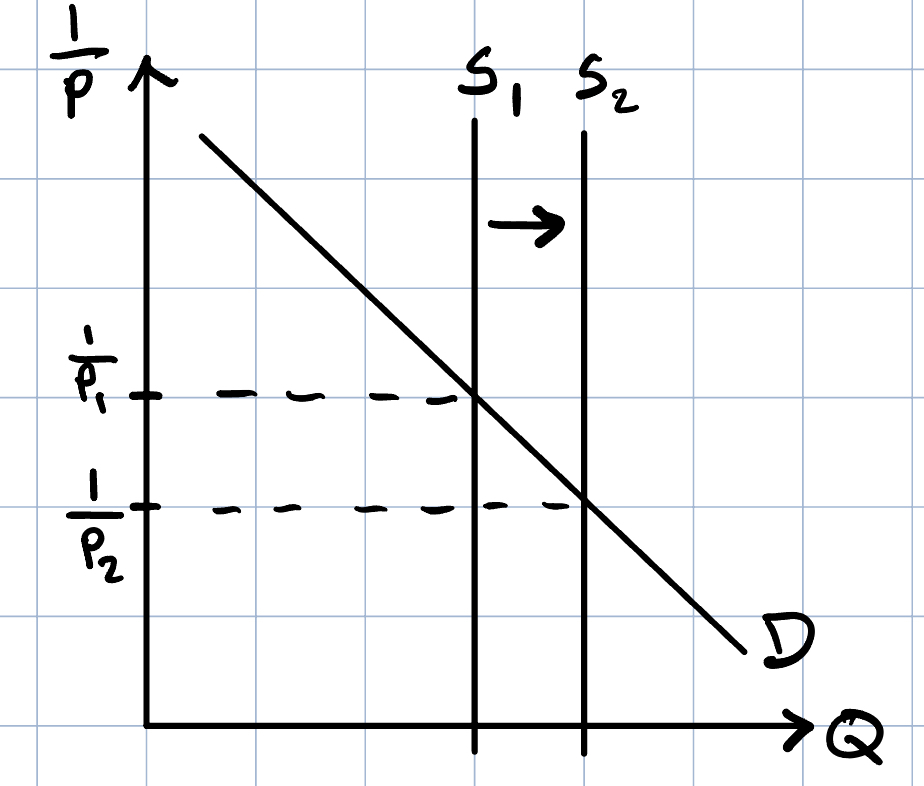
\includegraphics[width = 0.5\textwidth]{qfr2}
	\end{center}

\item The measurement of nominal variables includes the price level. The measurement of real variables does not. For example, nominal GDP changes depending on the price of current production. Real GDP does not. Similarly, the nominal interest rate changes depending on inflation. The real interest rate does not. The principle of monetary neutrality posits that the quantity of money only affects nominal variables.

\end{enumerate}

\section*{Problems and Applications}

\begin{enumerate}

\setcounter{enumi}{1}

\item

	\begin{enumerate}
	
	\item If people don't need to hold as much cash, the demand for money will decrease (shift left).
	
	\item If the Fed doesn't respond, then the value of money will decrease. When the value of money decreases, the price level increases.
	
		\begin{center}
		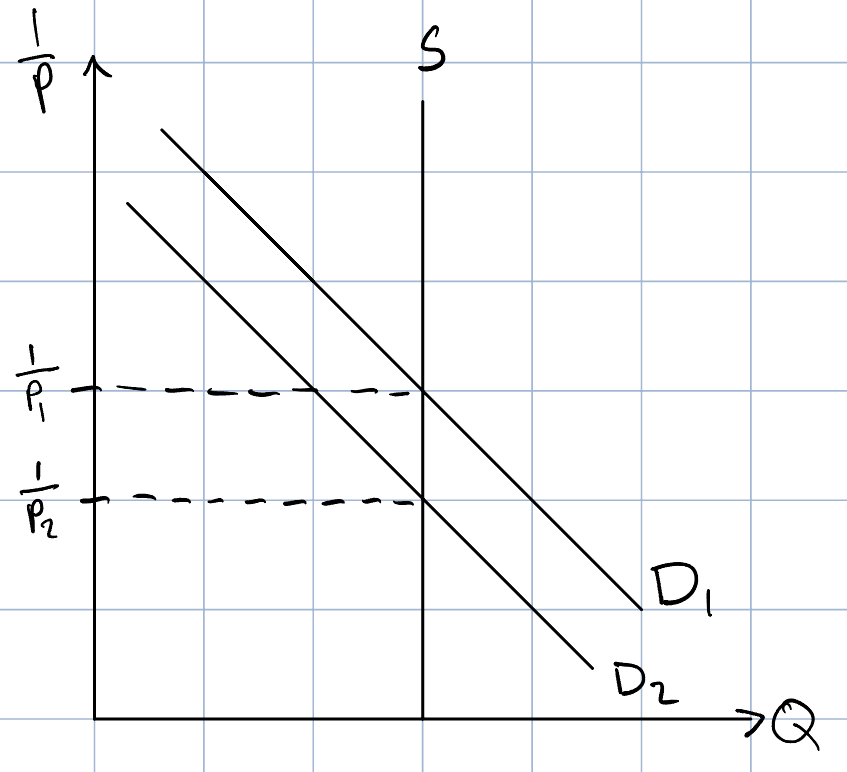
\includegraphics[width = 0.5\textwidth]{paa2b}
		\end{center}
	
	\item The Fed could keep the price level stable by decreasing the money supply. 
	
		\begin{center}
		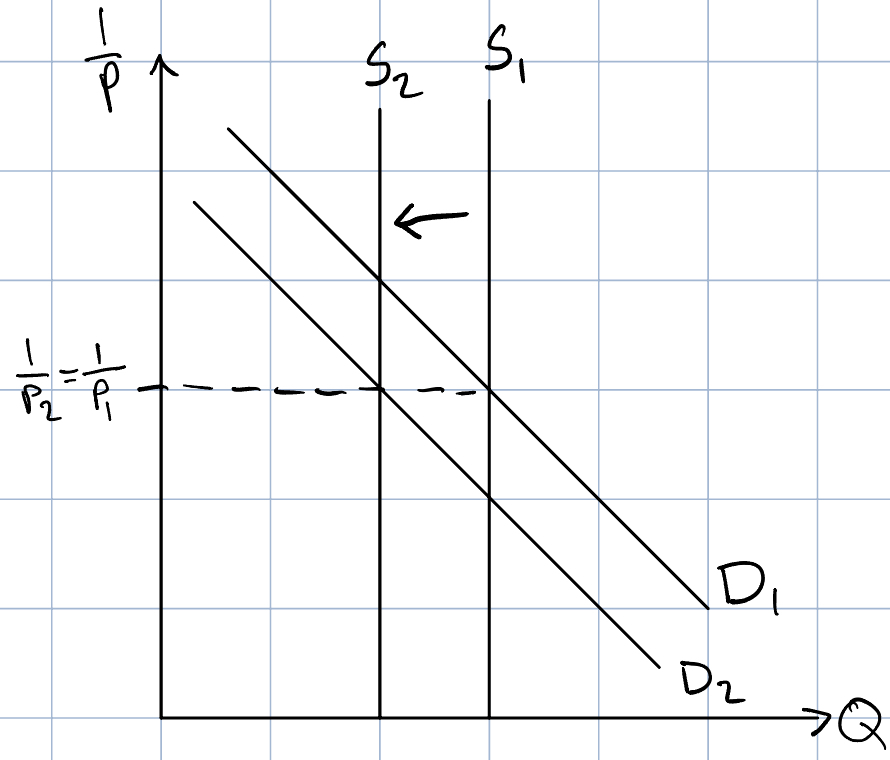
\includegraphics[width = 0.5\textwidth]{paa2c}
		\end{center}
	
	\end{enumerate}

\end{enumerate}

\end{document}